              
\documentclass[journal,onecolumn]{IEEEtran}
\usepackage{graphicx}
\setlength{\parindent}{0pt}

\ifCLASSINFOpdf
 
\else
 
\fi

% correct bad hyphenation here
\hyphenation{op-tical net-works semi-conduc-tor}


\begin{document}

\title{LAB 5 : Linux Command Line Utilities Simulator in C Programming}

\author{Nirajan~Bekoju \\ PUL076BCT039 \\ $2^{nd}$ March, 2023}

% The paper headers
\markboth{LAB 5 : Linux Command Line Utilities Simulator in C Programming}%
{Shell \MakeLowercase{\textit{et al.}}: Bare Demo of IEEEtran.cls for IEEE Journals}

% make the title area
\maketitle

\IEEEpeerreviewmaketitle

\section{Introduction}
A Linux Command Line Utilities Simulator in C Programming is a collection of programs that simulate the behavior of various Linux commands in a command line environment. The purpose of this simulator is to provide a way for users to learn and practice using Linux commands without having to install Linux or access a Linux terminal.

Each program in the simulator is written in the C programming language and emulates the functionality of a specific Linux command. For example, one program may simulate the behavior of the "ls" command, while another program may simulate the behavior of the "cd" command.

The programs in the simulator typically use standard input and output to communicate with the user, allowing the user to input command line arguments and see the output of the simulated command. The programs may also use system calls and libraries to access the file system and perform other operations required by the simulated command.

The Linux Command Line Utilities Simulator in C Programming can be a useful tool for individuals who are new to Linux and want to learn how to use Linux commands, as well as for experienced Linux users who want to test out different command options or troubleshoot issues in a safe and controlled environment. It can also be used by educators as a teaching tool in computer science or information technology courses.

\section{Implementation of ls Command}
\textbf{Aim : } To write a C program to simulate the operation of “ls” command in Unix.

\textbf{Algorithm : }
\begin{list}{}{}
  \item STEP 1 : Check if the number of command line arguments is less than 2. If
  yes, Print error and exit.
  \item STEP 2 : Check if the second argument (i.e. directory to be listed) is valid or not. If not
  then exit.
  \item STEP 3 : Print the content of the directory
  \item STEP 4 : Close the directory entry file.
\end{list}

\textbf{Program : }
\begin{verbatim}
  #include <stdio.h>
  #include <sys/types.h>
  #include <dirent.h>
  
  // struct dirent {
  //     ino_t          d_ino;       /* Inode number */
  //     off_t          d_off;       /* Not an offset; see below */
  //     unsigned short d_reclen;    /* Length of this record */
  //     unsigned char  d_type;      /* Type of file; not supported
  //                                     by all filesystem types */
  //     char           d_name[256]; /* Null-terminated filename */
  // };
  
  int main(int argc, char *argv[]){
      DIR *dp;
  
      struct dirent *dirp;
  
      if(argc < 2){
          printf("\n You have provided only 1 argument \n");
          return -1;
      }
      dp = opendir(argv[1]);
      if(dp == NULL){
          printf("\n Cannot open %s file!\n", argv[1]);
          return -1;
      }
      dirp = readdir(dp);
      while (dirp != NULL)
      {
          printf("%s\n", dirp->d_name);
          dirp = readdir(dp);
      }
      closedir(dp);
  }
\end{verbatim}

The folder structure for "search" folder is as follow:
\newline

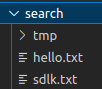
\includegraphics[scale=1.5]{search.png}


\textbf{Ouput :}
\begin{verbatim}
  $ ./ls search

  tmp
  hello.txt
  sdlk.txt
  .
  ..
\end{verbatim}




\section{Conclusion}
In this lab, we studied how we can simulate the Linux Command Line Utilities usinig C programming. And we also learn the basic of dirent in c programming.

In C programming language, the dirent.h header file provides a standard interface for accessing directory entries. The directory entry structure, struct dirent, is defined in this header file.

The struct dirent contains information about each directory entry, including the file name, the file type, and the file size. Here's an example of the struct definition:

\begin{verbatim}
  struct dirent {
    ino_t          d_ino;       /* inode number */
    off_t          d_off;       /* offset to the next dirent */
    unsigned short d_reclen;    /* length of this record */
    unsigned char  d_type;      /* type of file; not supported by 
                                    all file system types */
    char           d_name[256]; /* filename */
  };
\end{verbatim}

The d$\_$ino field is the inode number of the directory entry, which is a unique identifier for the file within the file system. The d$\_$off field is the offset to the next directory entry in the directory stream. The d$\_$reclen field is the length of the directory entry record, and the d$\_$type field indicates the type of the file, such as a regular file, a directory, a symbolic link, or other file types. The d$\_$name field is a character array that contains the name of the directory entry. It is limited to 256 characters to ensure compatibility across different file systems.

The dirent.h header file provides a set of functions for working with directory entries, including opendir(), readdir(), and closedir(). These functions allow you to open a directory stream, read the directory entries, and close the directory stream when you are done.

Overall, dirent in C provides a simple and standardized way to work with directory entries in a cross-platform manner.

\end{document}